\documentclass[
  man,
  colorlinks=true,linkcolor=blue,citecolor=blue,urlcolor=blue]{apa7}

% TODO: Add custom LaTeX header directives here
\makeatletter
\renewcommand{\paragraph}{\@startsection{paragraph}{4}{\parindent}%
	{0\baselineskip \@plus 0.2ex \@minus 0.2ex}%
	{-.5em}%
	{\normalfont\normalsize\bfseries\typesectitle}}

\renewcommand{\subparagraph}[1]{\@startsection{subparagraph}{5}{0.5em}%
	{0\baselineskip \@plus 0.2ex \@minus 0.2ex}%
	{-\z@\relax}%
	{\normalfont\normalsize\bfseries\itshape\hspace{\parindent}{#1}\textit{\addperi}}{\relax}}
\makeatother

\makeatletter\makeatother\makeatletter\makeatother\makeatletter\@ifpackageloaded{caption}{}{\usepackage{caption}}\AtBeginDocument{%
\ifdefined\contentsname
  \renewcommand*\contentsname{Table of contents}
\else
  \newcommand\contentsname{Table of contents}
\fi
\ifdefined\listfigurename
  \renewcommand*\listfigurename{List of Figures}
\else
  \newcommand\listfigurename{List of Figures}
\fi
\ifdefined\listtablename
  \renewcommand*\listtablename{List of Tables}
\else
  \newcommand\listtablename{List of Tables}
\fi
\ifdefined\figurename
  \renewcommand*\figurename{Figure}
\else
  \newcommand\figurename{Figure}
\fi
\ifdefined\tablename
  \renewcommand*\tablename{Table}
\else
  \newcommand\tablename{Table}
\fi
}\@ifpackageloaded{float}{}{\usepackage{float}}
\floatstyle{ruled}
\@ifundefined{c@chapter}{\newfloat{codelisting}{h}{lop}}{\newfloat{codelisting}{h}{lop}[chapter]}
\floatname{codelisting}{Listing}\newcommand*\listoflistings{\listof{codelisting}{List of Listings}}\makeatother\makeatletter\@ifpackageloaded{caption}{}{\usepackage{caption}}
\@ifpackageloaded{subcaption}{}{\usepackage{subcaption}}\makeatother\makeatletter\@ifpackageloaded{tcolorbox}{}{\usepackage[skins,breakable]{tcolorbox}}\makeatother\makeatletter\@ifundefined{shadecolor}{\definecolor{shadecolor}{rgb}{.97, .97, .97}}\makeatother\makeatletter\makeatother\makeatletter\makeatother



% \usepackage[style=apa,backend=biber]{biblatex}
% % \addbibresource{bibliography.bib}
% 
\newlength{\cslhangindent}
\setlength{\cslhangindent}{1.5em}
\newlength{\csllabelwidth}
\setlength{\csllabelwidth}{3em}
\newlength{\cslentryspacingunit} % times entry-spacing
\setlength{\cslentryspacingunit}{\parskip}
\newenvironment{CSLReferences}[2] % #1 hanging-ident, #2 entry spacing
 {% don't indent paragraphs
  \setlength{\parindent}{0pt}
  % turn on hanging indent if param 1 is 1
  \ifodd #1
  \let\oldpar\par
  \def\par{\hangindent=\cslhangindent\oldpar}
  \fi
  % set entry spacing
  \setlength{\parskip}{#2\cslentryspacingunit}
 }%
 {}
\usepackage{calc}
\newcommand{\CSLBlock}[1]{#1\hfill\break}
\newcommand{\CSLLeftMargin}[1]{\parbox[t]{\csllabelwidth}{#1}}
\newcommand{\CSLRightInline}[1]{\parbox[t]{\linewidth - \csllabelwidth}{#1}\break}
\newcommand{\CSLIndent}[1]{\hspace{\cslhangindent}#1}

\title{Collecting Concurrent Validity, Expert-Rater Agreement, and
Inter/Intra-Rater Reliability for the ANONYMIZED}
\shorttitle{Template for the APAquarto Format}




\authorsnames[{1},{2},{3}]{
Mackinsey Woolever,Ovande Furtado Jr,Jere D. Gallagher
}

\authorsaffiliations{
{Department of Kinesiology, California State University,
Northridge},{Department of Kinesiology, California State University,
Northridge},{University of Pittsburgh}}

\date{}
\abstract{Fundamental movement skills (FMS) are considered the building
blocks for developing specialized sports skills. In addition,
fundamental movement skill competency has been linked to decreased
levels of obesity and increased levels of physical activity/sports
participation. Thus, assessing FMS development is crucial. This study
aimed to collect evidence for concurrent validity, expert-rater
agreement, and inter/intra-rater reliability for the ANONYMIZED.
Participants were 34 children ages 5-10 years and 5 raters. Partial
Pearson correlations comparing the scores of both tests indicate a
moderate to strong correlation for locomotion (rxy.z =.52, p \textless{}
.01), object manipulation (rxy.z =.59, p \textless{} .001), and total
scores (rxy.z =.63, p \textless{} .001). The expert-rater agreement was
assessed by comparing the live scores of five raters with those of an
expert. Inter-rater reliability was assessed by comparing the scores
across the five raters. Intra- rater reliability was assessed by
comparing each rater's live and video scores. Weighted kappa scores
ranged from .51 to .83, .50 to .89, and .60 to .87 for expert-rater
agreement and inter and intra-rater reliability, respectively. These
results provide further validity and reliability evidence for the
FG-COMPASSANONYMIZED. Further studies involving children with different
ethnic backgrounds and larger sample size are recommended. ADD
LIMITATIONS HERE.}
% % \addbibresource{bibliography.bib}
% 
\keywords{Assessment, Fundamental Movement Skills, Children, Movement
Competence}

\authornote{\par{\addORCIDlink{Mackinsey
Woolever}{0000-0000-0000-0000}}\par{\addORCIDlink{Ovande Furtado
Jr}{0000-0003-3847-6314}}
\par{ Jere D. Gallagher is deceased.}
\par{        }
\par{Correspondence concerning this article should be addressed to Ovande
Furtado Jr, Department of Kinesiology, California State University,
Northridge, 18111 Nordhoff
St, Northridge, CA 91330-8287, Email: ovande@gmail.com (818-564-7507)}}


\begin{document}
\maketitle
\ifdefined\Shaded\renewenvironment{Shaded}{\begin{tcolorbox}[enhanced, sharp corners, frame hidden, interior hidden, borderline west={3pt}{0pt}{shadecolor}, boxrule=0pt, breakable]}{\end{tcolorbox}}\fi
Proficiency in fundamental movement skills (FMS) is critical for young
children and may positively or negatively affect their development and
lifestyle. Motor competence is a significant factor in participation in
physical activities (Castelli \& Valley, 2007). Perceived motor
competence has been shown to have a positive relationship with
proficiency in FMS in children and adolescents (Woods et al., 2007).
Physical activity participation is positively associated with
proficiency in FMS, especially if the activities are moderate to
vigorous (Bellows et al., 2013; Fisher et al., 2005; Lemos, 2012;
McKenzie et al., 2002) and inversely associated with obesity (Bayer et
al., 2009; Graf et al., 2004; Lopes et al., 2012). Studies have shown
that children who lack motor skill proficiency are less physically
active (Fisher et al., 2005; McKenzie et al., 2002) and are more likely
to be overweight or obese (Cliff et al., 2012).

Due to the critical role mastering gross motor skills has on a child's
lifespan, assessing FMS development is critical for preschool and
elementary school-aged children. According to Ulrich (2000), childhood
education often overlooks gross motor skills. Assessment tools are
designed to detect motor delays that may range from minor to severe. If
not addressed early, delays in motor skill development may hinder future
gross motor skill development (Ulrich, 2000), and likely impact the
acquisition of specialized skills (Gabbard, 2021). A developmental delay
is defined by Provost et al. (2000) as a difference of 25\% or more
between a child's actual age and their developmental age. If a motor
delay is detected early, practitioners, parents, and educators can
implement strategies to help the child.

There are various tools available to evaluate the progress of
fundamental movement skills (Cools et al., 2009). However, these tools
are not typically meant to be used in real time by a single
practitioner. Usually, the administrators need to film the performances
and rate them later. It would be more convenient to have an assessment
tool that allows professionals to assess children without recording
their performances. The Test of Gross Motor Development - Second Edition
(TGMD-2) is considered the gold standard for assessing FMS competency in
children between the ages of 3 and 10 years (Ulrich, 2000) and was used
as the criterion for the analysis of concurrent validity in this study.
The TGMD-2 has two gross motor subtests (locomotor and manipulative) and
assesses 12 skills. The FG-COMPASS was developed to assess gross motor
skill development in children between the ages of 5 and 10 (Furtado \&
Gallagher, 2012). The FG-COMPASS is similar to the TGMD-2 in that it
assesses locomotor and object manipulation skills as fundamental gross
motor skills. The FG-COMPASS is designed to be administered live by a
single practitioner without the need to video-record the performer.

It is essential to have a reliable and valid assessment tool to evaluate
gross motor development in school-age children. This helps identify any
potential motor delays and ensures typical development. So far, no
attempts have been made to compare the results of FG-COMPASS with those
of a criterion instrument like TGMD-2. Although there is evidence of
inter- and intra-rater reliability for FG-COMPASS (Furtado \& Gallagher,
2012, 2018), the agreement data were collected through video analysis,
not live performances. Therefore, this study aims to assess inter- and
intra-rater agreement in a live setting. Therefore, this study aimed to
collect criterion-related (concurrent) validity for the FG-COMPASS by
comparing its results with the results of the TGMD-2. In addition, this
study sought to collect further inter-, intra-, and expert-rater
reliability evidence for the FG-COMPASS from live assessments. Several
hypotheses were proposed for this study. We anticipated that there would
be at least a `good' agreement (ICC/kappa scores above 0.74) for the
locomotor (LFMS), manipulative (MFMS), and total test (TFMS) when
investigating concurrent validity, inter- and intra-rater reliability,
and expert-rater reliability for the FG-COMPASS.

\hypertarget{materials-and-methods}{%
\section{Materials and Methods}\label{materials-and-methods}}

\hypertarget{participants}{%
\subsection{Participants}\label{participants}}

A convenient sampling method was used to recruit participants for this
study. After Institutional Review Board approval, 41 children between
the ages of 5 and 10 were recruited. However, only 34 children, 22 girls
(M = 8.14, SD = 1.78) and 12 boys (M = 8.44, SD = 1.49), participated
fully. Three participants dropped out independently; two never attended
the assessment sessions; one was injured before the assessment, and one
child moved out of the state during the data collection. Informed
consent was obtained from each participant's parents or legal guardians
before their involvement in the study. One randomly selected
kindergarten through fourth-grade classroom received a recruitment
packet to control for an even distribution of age ranges. Recruitment
packets were given to additional classrooms if no consent forms were
returned. A participant was excluded from the study if he/she: 1) was
younger than 5 years or older than 10 years and 11 months; 2) had
developmental delays or disabilities that may have affected their motor
performance; 3) had no parental or verbal consent; or 4) had a ``yes''
response on any of the first five Physical Activity
Readiness-Questionnaire (PAR-Q) questions (Adams, 1999).

\hypertarget{measures}{%
\subsection{Measures}\label{measures}}

\hypertarget{tgmd-2}{%
\subsubsection{TGMD-2}\label{tgmd-2}}

The TGMD-2 (Ulrich, 2000) was used as the target test (gold standard)
for the concurrent validity analysis. The TGMD-2 measures twelve gross
motor skills (six locomotion and six object manipulation) in children
between 3 and 10 years old. The TGMD-2 assesses several performance
criteria focusing on different body components, such as the arms, legs,
and trunk. For example, a performance criterion for hopping is to have
``arms flexed and swing forward to produce force''. The child has two
attempts to complete each skill. If the performance criterion is
demonstrated during a trial, a score of 1 is awarded. If not, the child
receives a score of 0. After scoring the performance criterion for two
trials on each skill, the scores are added to obtain the overall raw
score for each subtest. Then, the raw scores for each subtest are
converted into standard scores, which can be compared to normative data.
By analyzing the standard scores from both subtests, age equivalents,
and percentiles can be determined. When added together, the standard
scores can be converted to a gross motor quotient value.

Several studies have been conducted to evaluate the validity and
reliability of the TGMD-2. The test has been found to have strong
construct validity, as it accurately measures the underlying theoretical
construct of gross motor development (Ulrich, 2000). Concurrent validity
has been established through correlations with other established motor
skill assessments, such as the Movement Assessment Battery for Children
(MABC) (Cools et al., 2009). The test-retest reliability of the TGMD-2
is high, with coefficients often exceeding 0.90 (Valentini \& Rudisill,
2004). Internal consistency has also been demonstrated, with Cronbach's
alpha values typically above 0.80 for locomotion and object manipulation
subtests (Wiart \& Darrah, 2001). Moreover, the TGMD-2 has been adapted
and validated for use in various cultural contexts, reflecting its
applicability across diverse populations (Barnett et al., 2009). The
standardization process of the TGMD-2 included a representative sample
of children in the United States, ensuring that the normative data were
relevant for the target age group.

\hypertarget{fg-compass}{%
\subsubsection{FG-COMPASS}\label{fg-compass}}

The FG-COMPASS is an evaluation tool designed for children aged 5 to 10
to assess their gross motor skills. These skills comprise three related
to locomotion and five related to object manipulation. When creating the
FG-COMPASS, Furtado and Gallagher (2012) proposed a novel approach to
developing FMS rating scales. This approach uses key performance
criteria as a decision tree and is described elsewhere (Furtado \&
Gallagher, 2012; Perez, 2018). The decision tree created for the skill
`Overhand Throw' using the authors' suggested method is shown in Figure
1. There are three types of nodes in the flowchart: decision nodes
(questions), chance nodes (yes or no), and end nodes (levels). Even
though multiple performance criteria can be proposed for a skill, the
suggested method only chooses three to form the skill's decision tree.
The decision nodes of the decision tree are then created from these
performance criteria in the form of questions. A discriminatory question
can be found in Figure 1's top decision node. To distinguish between
levels 1 and 4. (end nodes). If the chance node is `yes', the decision
is made to go in the direction on the right, and the observer is then
given a confirmatory question to see if the performer is proficient in
overhand throws at level 4 (the chance node is `yes'). The performer is
rated level 3 if the decision tree cannot confirm a level 4 (chance node
is `no'). The decision tree's left side serves the same function, except
it checks to see if the performer is at level 1. With only two
performance criteria considered when determining the proficiency levels
of performers, the decision-tree approach simplifies the evaluation of
live performances of fundamental movement skills. Multiple studies have
demonstrated evidence of validity and reliability for the FG-COMPASS.
This includes evidence for content-related validity
(\textbf{furtado2004?}), expert-rater agreement Furtado \& Gallagher
(2018), and intra- and inter-rater reliability (Furtado \& Gallagher,
2018).

{[}figure 1 here{]}

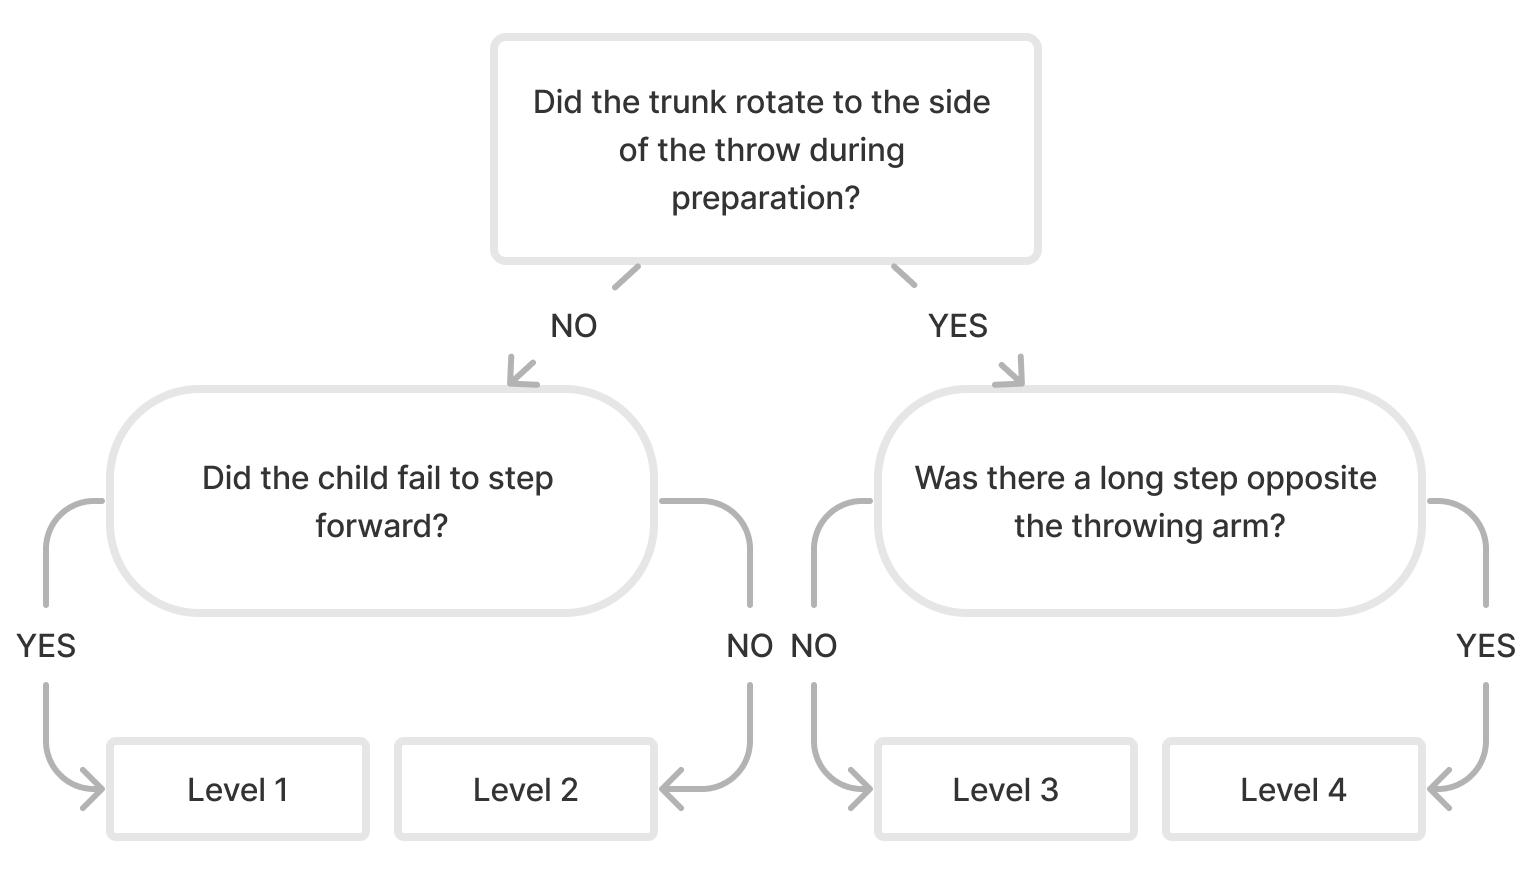
\includegraphics{images/fgcompass-dt-man-ot.png}

\hypertarget{research-assistants}{%
\subsection{Research Assistants}\label{research-assistants}}

Sixteen kinesiology undergraduate students were recruited as research
assistants. Ten of the sixteen students were recruited as raters, with
each instrument having five raters to complete the assessment of gross
motor skills. Once selected, the raters were randomly assigned to either
the TGMD-2 or the FG-COMPASS. Three students were test administrators
for the TGMD-2 and two for the FG-COMPASS. One student never attended
the site and was responsible for editing the videos. The training was
slightly different for each assessment tool. Each group of raters
underwent multiple training and review sessions before data collection.
In addition, the test administrators went through multiple training and
practice sessions on skill set-up, instructions, demonstrations, and
camera placement and handling before data collection.

\hypertarget{procedures}{%
\subsection{Procedures}\label{procedures}}

\hypertarget{data-collection}{%
\subsubsection{Data collection}\label{data-collection}}

Even though the TGMD-2 and the FG-COMPASS assess the same construct,
there are differences between the two tests. Nevertheless, some shared
practices were utilized during the administration of both assessments.
Participants were assessed during their morning or lunch recess, and all
students completed both tests. Before collecting data, the primary
investigator (PI) gave identification numbers to the participants. Upon
arrival at the testing site, they were directed to the TGMD-2 or
FG-COMPASS stations based on a randomized list. The process was repeated
weekly to prevent any learning effects that could result from measuring
the same skill multiple times. Once the participants completed the
initial assessment at either the TGMD-2 or FG-COMPASS stations, they
proceeded to the second station for the second evaluation. Depending on
the circumstances, some participants were required to perform multiple
skills on both instruments, requiring them to switch between the two
stations.

Each week, the test administrators in charge of the TGMD-2 testing
attended the site. They followed the procedures outlined in the test's
user manual (Ulrich, 2000), and all performances were recorded on video.
The raters assigned to the TGMD-2 were then invited to the lab to
evaluate the recorded videos of the TGMD-2 performances. The raters
assigned to the FG-COMPASS assessed the skills live, on-site. In
addition, the performances were recorded on video. This served to
evaluate intra-rater reliability for the FG-COMPASS. For both tests,
participants completed one practice trial and three testing trials for
each skill.

\hypertarget{data-analysis}{%
\subsection{Data Analysis}\label{data-analysis}}

Concurrent validity was investigated with the intraclass correlation
coefficient (ICC, 2, k) and Bland Altman plots . Weighted kappa
statistics were used to evaluate the inter- and intra-rater reliability
of the FG-COMPASS, as well as the agreement between the expert and
raters. The ICC is intended to assess rating reliability by comparing
the variability of different ratings of the same participant to the
total variation across all ratings and all participants {[}McGraw and
Wong (1996){]}. The Bland-Altman technique {[}Bland and Altman (1986){]}
involves measuring the agreement between two quantitative measurements
by examining the average difference and creating boundaries of
agreement, which is preferred over correlational techniques {[}Giavarina
(2015){]}. Using the weighted Kappa index (Fleiss \& Cohen, 1973) is
advised when more than two coders independently assess an entity into
three or more distinct (ordinal level) categories. Weighted kappa, in
contrast to kappa, assigns various weights based on the degree of
disagreement. The weighted kappa and ICC values were interpreted as
follows: \textgreater0.75 excellent, 0.74-0.60 good, 0.59-0.40 fair, and
\textless0.40 poor (Cicchetti, 1994). This study employed a
cross-sectional design, and all statistical analyses were performed
using the statistical package jamovi (The jamovi project, 2022).

\hypertarget{results}{%
\section{Results}\label{results}}

\hypertarget{concurrent-validity}{%
\subsection{Concurrent Validity}\label{concurrent-validity}}

The agreement between the FG-COMPASS and TGMD-2 (see
Table~\ref{apatb-table1}) was evaluated using the intraclass correlation
coefficient and Bland-Altman analysis for LFMS, MFMS, and TFMS. The ICC
for the LFMS subtest was 0.68, indicating a `good' agreement between the
two tests. The Bland-Altman analysis revealed a mean bias close to zero.
`Excellent' agreement was observed for the MFMS subtest, with an ICC of
0.89 and Bland-Altman bias close to zero. The TFMS also demonstrated
`excellent' agreement, with an ICC of 0.89 and Bland-Altman bias close
to zero.

\begin{table}
\caption{Concurrent Validity Analysis for FG-COMPASS}
\label{apatb-table1}

\begin{longtable}[]{@{}
  >{\raggedright\arraybackslash}p{(\columnwidth - 10\tabcolsep) * \real{0.1169}}
  >{\raggedright\arraybackslash}p{(\columnwidth - 10\tabcolsep) * \real{0.1364}}
  >{\raggedright\arraybackslash}p{(\columnwidth - 10\tabcolsep) * \real{0.1494}}
  >{\raggedright\arraybackslash}p{(\columnwidth - 10\tabcolsep) * \real{0.1429}}
  >{\raggedright\arraybackslash}p{(\columnwidth - 10\tabcolsep) * \real{0.2273}}
  >{\raggedright\arraybackslash}p{(\columnwidth - 10\tabcolsep) * \real{0.2273}}@{}}
\toprule\noalign{}
\begin{minipage}[b]{\linewidth}\raggedright
\end{minipage} & \begin{minipage}[b]{\linewidth}\raggedright
ICC (95\% CI)
\end{minipage} & \begin{minipage}[b]{\linewidth}\raggedright
F-Statistic (p-value)
\end{minipage} & \begin{minipage}[b]{\linewidth}\raggedright
Bias (95\% CI)
\end{minipage} & \begin{minipage}[b]{\linewidth}\raggedright
LLA (95\% CI)
\end{minipage} & \begin{minipage}[b]{\linewidth}\raggedright
ULA (95\% CI)
\end{minipage} \\
\midrule\noalign{}
\endhead
\bottomrule\noalign{}
\endlastfoot
\textbf{Locomotor} & 0.68 (0.350, 0.840) & 3.05 (0.001) & 1.73e−16
(−0.347, 0.347) & −1.95 (−2.547, −1.350) & 1.95 (1.350, 2.547) \\
\textbf{Manipulative} & 0.89 (0.779, 0.945) & 8.85 (\textless0.001) &
2.60e−16 (−0.222, 0.222) & −1.25 (−1.633, −0.865) & 1.25 (0.865,
1.633) \\
\textbf{Total test} & 0.89 (0.783, 0.946) & 9.00 (\textless0.001) &
−2.53e−16 (−0.221, 0.221) & −1.24 (−1.621, −0.859) & 1.24 (0.859,
1.621) \\
\end{longtable}

\textbackslash tablenote\{ICC:~Intraclass Correlation Coefficient (ICC,
2, k). Bias:~Mean difference between the two methods. LLA \& ULA:~95\%
lower and upper limits of agreement in the Bland-Altman analysis.\}

\textbackslash end\{table\}

\begin{verbatim}
:::




## Inter-Rater Reliability

The inter-rater reliability of the FG-COMPASS was assessed by comparing the live scores of all five raters involved in the study (see {apatb-table2}). Weighted kappa values were computed for each pair of raters, and then the mean was calculated to provide a single index of reliability [@light1971]. Weighted kappa values ranged from 0.42 to 0.93 (M = 0.66 SD = .15) for the LFMS subtest and from 0.31 to 0.93 (M = 0.77 SD = 0.15) for the MFMS subtest. The test's combined score (TFMS) was 0.72 (SD = 0.15). The resulting weighted kappa indicates 'good' agreement for the LFMS, MFMS subtests, and the total test (TFMS).




::: {.cell apa-cap='Weighted Kappa Statistics for the Inter-Rater Analysis' apa-note='_N_ = ???. LFMS = Locomotor Subtest. MFMS = Manipulative Subtest. TFMS = Locomotor and Manipulative scores combined. <br/> Asterisks indicate major disagreement between rater 5 and all other raters.'}
```{=latex}
\begin{table}
\caption{Weighted Kappa Statistics for the Inter-Rater Analysis}
\label{apatb-table2}
\end{verbatim}

\begin{longtable}[]{@{}
  >{\raggedright\arraybackslash}p{(\columnwidth - 26\tabcolsep) * \real{0.1471}}
  >{\raggedright\arraybackslash}p{(\columnwidth - 26\tabcolsep) * \real{0.1471}}
  >{\raggedright\arraybackslash}p{(\columnwidth - 26\tabcolsep) * \real{0.0588}}
  >{\raggedright\arraybackslash}p{(\columnwidth - 26\tabcolsep) * \real{0.0588}}
  >{\raggedright\arraybackslash}p{(\columnwidth - 26\tabcolsep) * \real{0.0588}}
  >{\raggedright\arraybackslash}p{(\columnwidth - 26\tabcolsep) * \real{0.0588}}
  >{\raggedright\arraybackslash}p{(\columnwidth - 26\tabcolsep) * \real{0.0588}}
  >{\raggedright\arraybackslash}p{(\columnwidth - 26\tabcolsep) * \real{0.0588}}
  >{\raggedright\arraybackslash}p{(\columnwidth - 26\tabcolsep) * \real{0.0588}}
  >{\raggedright\arraybackslash}p{(\columnwidth - 26\tabcolsep) * \real{0.0588}}
  >{\raggedright\arraybackslash}p{(\columnwidth - 26\tabcolsep) * \real{0.0588}}
  >{\raggedright\arraybackslash}p{(\columnwidth - 26\tabcolsep) * \real{0.0588}}
  >{\raggedright\arraybackslash}p{(\columnwidth - 26\tabcolsep) * \real{0.0588}}
  >{\raggedright\arraybackslash}p{(\columnwidth - 26\tabcolsep) * \real{0.0588}}@{}}
\toprule\noalign{}
\begin{minipage}[b]{\linewidth}\raggedright
\end{minipage} & \begin{minipage}[b]{\linewidth}\raggedright
Skill
\end{minipage} & \begin{minipage}[b]{\linewidth}\raggedright
1x2
\end{minipage} & \begin{minipage}[b]{\linewidth}\raggedright
1x3
\end{minipage} & \begin{minipage}[b]{\linewidth}\raggedright
1x4
\end{minipage} & \begin{minipage}[b]{\linewidth}\raggedright
1x5
\end{minipage} & \begin{minipage}[b]{\linewidth}\raggedright
2x3
\end{minipage} & \begin{minipage}[b]{\linewidth}\raggedright
2x4
\end{minipage} & \begin{minipage}[b]{\linewidth}\raggedright
2x5
\end{minipage} & \begin{minipage}[b]{\linewidth}\raggedright
3x4
\end{minipage} & \begin{minipage}[b]{\linewidth}\raggedright
3x5
\end{minipage} & \begin{minipage}[b]{\linewidth}\raggedright
4x5
\end{minipage} & \begin{minipage}[b]{\linewidth}\raggedright
Mean
\end{minipage} & \begin{minipage}[b]{\linewidth}\raggedright
SD
\end{minipage} \\
\midrule\noalign{}
\endhead
\bottomrule\noalign{}
\endlastfoot
\textbf{LFMS} & & & & & & & & & & & & \textbf{.66} & .15 \\
& Hop & .56 & .43 & .43 & .50 & .42 & .49 & .46 & .53 & .64 & .52 & .50
& .07 \\
& Jump & .93 & .91 & .70 & .65 & .84 & .73 & .62 & .61 & .61 & .69 & .73
& .12 \\
& Skip & .78 & .74 & .60 & .63 & .87 & .77 & .76 & .69 & .71 & .83 & .74
& .08 \\
\textbf{MFMS} & & & & & & & & & & & & \textbf{.77} & .15 \\
& Throw & .85 & .79 & .85 & .45* & .80 & .73 & .35* & .71 & .31* & .40*
& .62 & .22 \\
& Kick & .83 & .68 & .64 & .82 & .63 & .59 & .73 & .50 & .72 & .64 & .68
& .10 \\
& Dribble & .86 & .87 & .83 & .92 & .88 & .84 & .91 & .88 & .93 & .93 &
.89 & .04 \\
& Catch & .87 & .91 & .87 & .90 & .83 & .84 & .90 & .80 & .80 & .89 &
.86 & .04 \\
& Strike & .81 & .80 & .72 & .72 & .87 & .80 & .80 & .69 & .78 & .79 &
.78 & .05 \\
\textbf{TFMS} & & & & & & & & & & & & \textbf{.72} & .15 \\
\end{longtable}

\tablenote{_N_ = ???. LFMS = Locomotor Subtest. MFMS = Manipulative Subtest. TFMS = Locomotor and Manipulative scores combined. <br/> Asterisks indicate major disagreement between rater 5 and all other raters.}

\end{table}

\hypertarget{intra-rater-reliability-for-the-fg-compass}{%
\subsection{Intra-rater reliability for the
FG-COMPASS}\label{intra-rater-reliability-for-the-fg-compass}}

We evaluated the consistency of ratings by comparing live assessments
with those obtained through video assessments (see
Table~\ref{apatb-table3}). Of particular interest is `IR1', which
compares the ratings obtained from live assessments with those from
recorded performances (time 1), which took place one week after the live
assessment at the site. Additionally, we included ratings from a second
video assessment and compared it with the live assessment (IR2) and the
first video assessment (IR3). In Table~\ref{apatb-table4}, we provide
the mean and standard deviation scores for each intra-rater comparison
across all five raters. Scores ranged from 0.50 to 0.89, indicating
agreement from `fair' to `excellent' (Cicchetti, 1994).

\newpage{}

\begin{table}
\caption{Intra-Rater Agreement Measured by Weighted Kappa Coefficients Across Different Skills}
\label{apatb-table3}

\begin{longtable}[]{@{}
  >{\raggedright\arraybackslash}p{(\columnwidth - 30\tabcolsep) * \real{0.0441}}
  >{\raggedright\arraybackslash}p{(\columnwidth - 30\tabcolsep) * \real{0.0637}}
  >{\raggedright\arraybackslash}p{(\columnwidth - 30\tabcolsep) * \real{0.0637}}
  >{\raggedright\arraybackslash}p{(\columnwidth - 30\tabcolsep) * \real{0.0637}}
  >{\raggedright\arraybackslash}p{(\columnwidth - 30\tabcolsep) * \real{0.0637}}
  >{\raggedright\arraybackslash}p{(\columnwidth - 30\tabcolsep) * \real{0.0637}}
  >{\raggedright\arraybackslash}p{(\columnwidth - 30\tabcolsep) * \real{0.0637}}
  >{\raggedright\arraybackslash}p{(\columnwidth - 30\tabcolsep) * \real{0.0637}}
  >{\raggedright\arraybackslash}p{(\columnwidth - 30\tabcolsep) * \real{0.0637}}
  >{\raggedright\arraybackslash}p{(\columnwidth - 30\tabcolsep) * \real{0.0637}}
  >{\raggedright\arraybackslash}p{(\columnwidth - 30\tabcolsep) * \real{0.0637}}
  >{\raggedright\arraybackslash}p{(\columnwidth - 30\tabcolsep) * \real{0.0637}}
  >{\raggedright\arraybackslash}p{(\columnwidth - 30\tabcolsep) * \real{0.0637}}
  >{\raggedright\arraybackslash}p{(\columnwidth - 30\tabcolsep) * \real{0.0637}}
  >{\raggedright\arraybackslash}p{(\columnwidth - 30\tabcolsep) * \real{0.0637}}
  >{\raggedright\arraybackslash}p{(\columnwidth - 30\tabcolsep) * \real{0.0637}}@{}}
\toprule\noalign{}
\begin{minipage}[b]{\linewidth}\raggedright
\end{minipage} & \begin{minipage}[b]{\linewidth}\raggedright
Rater 1
\end{minipage} & \begin{minipage}[b]{\linewidth}\raggedright
Rater 2
\end{minipage} & \begin{minipage}[b]{\linewidth}\raggedright
Rater 3
\end{minipage} & \begin{minipage}[b]{\linewidth}\raggedright
Rater 4
\end{minipage} & \begin{minipage}[b]{\linewidth}\raggedright
Rater 5
\end{minipage} & \begin{minipage}[b]{\linewidth}\raggedright
\end{minipage} & \begin{minipage}[b]{\linewidth}\raggedright
\end{minipage} & \begin{minipage}[b]{\linewidth}\raggedright
\end{minipage} & \begin{minipage}[b]{\linewidth}\raggedright
\end{minipage} & \begin{minipage}[b]{\linewidth}\raggedright
\end{minipage} & \begin{minipage}[b]{\linewidth}\raggedright
\end{minipage} & \begin{minipage}[b]{\linewidth}\raggedright
\end{minipage} & \begin{minipage}[b]{\linewidth}\raggedright
\end{minipage} & \begin{minipage}[b]{\linewidth}\raggedright
\end{minipage} & \begin{minipage}[b]{\linewidth}\raggedright
\end{minipage} \\
\midrule\noalign{}
\endhead
\bottomrule\noalign{}
\endlastfoot
& IR1 & IR2 & IR3 & IR1 & IR2 & IR3 & IR1 & IR2 & IR3 & IR1 & IR2 & IR3
& IR1 & IR2 & IR3 \\
Hop (17) & 0.72 & 0.83 & 0.89 & 0.44 & 0.55 & 0.75 & 0.64 & 0.62 & 0.88
& 0.69 & 0.40 & 0.62 & 0.84 & 0.62 & 0.80 \\
Jump (18) & 0.56 & 0.49 & 0.83 & 0.46 & 0.68 & 0.39 & 0.74 & 0.38 & 0.49
& 0.56 & 0.28 & 0.56 & 0.67 & 0.67 & 1.00 \\
Skip (18) & 0.96 & 0.96 & 1.00 & 0.94 & 0.78 & 0.86 & 0.92 & 0.86 & 0.89
& 0.51 & 0.68 & 0.86 & 0.66 & 0.52 & 0.83 \\
Throw (18) & 0.80 & 0.52 & 0.53 & 0.63 & 0.62 & 0.97 & 0.52 & 0.54 &
0.60 & 0.69 & 0.76 & 0.70 & 0.54 & 0.66 & 0.86 \\
Kick (19) & 0.72 & 0.68 & 0.78 & 0.66 & 0.60 & 0.76 & 0.80 & 0.70 & 0.74
& 0.74 & 0.64 & 0.72 & 0.64 & 0.62 & 0.80 \\
Dribble (17) & 0.86 & 0.80 & 0.82 & 0.70 & 0.78 & 0.86 & 0.66 & 0.60 &
0.82 & 0.76 & 0.68 & 0.74 & 0.60 & 0.64 & 0.68 \\
Catch (20) & 0.68 & 0.62 & 0.86 & 0.86 & 0.66 & 0.80 & 0.76 & 0.78 &
0.82 & 0.66 & 0.60 & 0.78 & 0.84 & 0.88 & 0.88 \\
Strike (20) & 0.62 & 0.56 & 0.60 & 0.74 & 0.70 & 0.70 & 0.64 & 0.64 &
0.64 & 0.74 & 0.68 & 0.68 & 0.70 & 0.62 & 0.78 \\
\end{longtable}

\tablenote{Quadratic weighted kappa values range from -1 to 1. IR1, IR2, IR3 represent three different comparison pairs:\ IR1 compares the ratings from the live performances with the recorded video (time 1), IR2 compares ratings from the live performances with the recorded video (time 2), and IR3 compares the ratings from the recorded performances from time 1 and time 2. Sample sizes for each skill are provided in parentheses next to the skill name. Rater 1 to Rater 5 represent five different individuals who rated the performances.}

\end{table}

\newpage{}

\begin{table}
\caption{Summary of Quadratic Weighted Kappa for Intra-Rater Comparisons Across Motor Skills}
\label{apatb-table4}

\begin{longtable}[]{@{}llll@{}}
\toprule\noalign{}
Skill & IR1 Mean (SD) & IR2 Mean (SD) & IR3 Mean (SD) \\
\midrule\noalign{}
\endhead
\bottomrule\noalign{}
\endlastfoot
LFMS & \textbf{0.69} & 0.62 & 0.78 \\
Hop & 0.67 (0.13) & 0.60 (0.14) & 0.79 (0.10) \\
Jump & 0.60 (0.10) & 0.50 (0.16) & 0.65 (0.23) \\
Skip & 0.80 (0.18) & 0.76 (0.15) & 0.89 (0.06) \\
MFMS & \textbf{0.70} & 0.66 & 0.76 \\
Throw & 0.64 (0.10) & 0.62 (0.09) & 0.73 (0.16) \\
Kick & 0.71 (0.06) & 0.65 (0.04) & 0.76 (0.03) \\
Dribble & 0.72 (0.09) & 0.70 (0.08) & 0.78 (0.06) \\
Catch & 0.76 (0.08) & 0.71 (0.11) & 0.83 (0.04) \\
Strike & 0.69 (0.05) & 0.64 (0.05) & 0.68 (0.06) \\
TFMS & \textbf{0.70} & 0.64 & 0.77 \\
\end{longtable}

\tablenote{IR1, IR2, IR3:\ Represent different inter-rater comparisons (e.g., live vs. video 1, live vs. video 2, video 1 vs. video 2). Mean:\ The average of the quadratic weighted kappa values for each scenario across all raters and skills. SD:\ The standard deviation of the quadratic weighted kappa values for each scenario across all raters and skills.}

\end{table}

\hypertarget{expert-rater-agreement-for-the-fg-compass}{%
\subsection{Expert-Rater Agreement for the
FG-COMPASS}\label{expert-rater-agreement-for-the-fg-compass}}

The study aimed to assess the level of agreement between raters and
expert ratings for the FG-COMPASS. The live ratings of five raters were
compared with the expert's video scores. The results showed that the
level of agreement varied across the skills assessed. For `Hop', the
agreement ranged from `fair' to `excellent', with a mean kappa value of
0.67. For `Skip', the agreement was more varied, with kappa values
ranging from `poor' to `excellent'. In the MFMS subtest, the agreement
was considered `excellent'. For `Throw', the agreement ranged from good
to excellent, with a mean kappa value of 0.75. For `Dribble', all raters
showed `excellent' agreement, with kappa values ranging from 0.77 to
0.94 and a mean kappa of 0.86. For `Catch', the agreement was
`excellent', with a mean kappa value of 0.83. For `Strike', the
agreement was `fair' to `good' with kappa values ranging from 0.40 to
0.61 and a mean kappa of 0.51. Considering all skills (TFMS), the mean
kappa value was 0.70, indicating `good' agreement across all skills when
considering all raters.

\begin{table}
\caption{Weighted Kappa Scores between Raters and an Expert}
\label{apatb-table5}

\begin{longtable}[]{@{}
  >{\raggedright\arraybackslash}p{(\columnwidth - 16\tabcolsep) * \real{0.0876}}
  >{\raggedright\arraybackslash}p{(\columnwidth - 16\tabcolsep) * \real{0.0949}}
  >{\raggedright\arraybackslash}p{(\columnwidth - 16\tabcolsep) * \real{0.1387}}
  >{\raggedright\arraybackslash}p{(\columnwidth - 16\tabcolsep) * \real{0.1387}}
  >{\raggedright\arraybackslash}p{(\columnwidth - 16\tabcolsep) * \real{0.1387}}
  >{\raggedright\arraybackslash}p{(\columnwidth - 16\tabcolsep) * \real{0.1460}}
  >{\raggedright\arraybackslash}p{(\columnwidth - 16\tabcolsep) * \real{0.1460}}
  >{\raggedright\arraybackslash}p{(\columnwidth - 16\tabcolsep) * \real{0.0584}}
  >{\raggedright\arraybackslash}p{(\columnwidth - 16\tabcolsep) * \real{0.0511}}@{}}
\toprule\noalign{}
\begin{minipage}[b]{\linewidth}\raggedright
\end{minipage} & \begin{minipage}[b]{\linewidth}\raggedright
Skill
\end{minipage} & \begin{minipage}[b]{\linewidth}\raggedright
Rater 1
\end{minipage} & \begin{minipage}[b]{\linewidth}\raggedright
Rater 2
\end{minipage} & \begin{minipage}[b]{\linewidth}\raggedright
Rater 3
\end{minipage} & \begin{minipage}[b]{\linewidth}\raggedright
Rater 4
\end{minipage} & \begin{minipage}[b]{\linewidth}\raggedright
Rater 5
\end{minipage} & \begin{minipage}[b]{\linewidth}\raggedright
Mean
\end{minipage} & \begin{minipage}[b]{\linewidth}\raggedright
SD
\end{minipage} \\
\midrule\noalign{}
\endhead
\bottomrule\noalign{}
\endlastfoot
LFMS & & & & & & & \textbf{0.64} & 0.12 \\
& Hop (17) & 0.71 (0.39, 0.90) & 0.77 (0.55, 0.87) & 0.50 (0.14, 0.73) &
0.65 (0.32, 0.90) & 0.70 (0.36, 0.88) & 0.67 & 0.09 \\
& Jump (18) & 0.74 (0.21, 1.00) & 0.83 (0.44, 1.00) & 0.78 (0.28, 1.00)
& 0.75 (0.44, 0.93) & 0.57 (0.18, 0.89) & 0.73 & 0.09 \\
& Skip (18) & 0.67 (0.37, 0.89) & 0.76 (0.36, 0.96) & 0.59 (0.26, 0.92)
& 0.29 (-0.06, 0.66) & 0.35 (-0.02, 0.72) & 0.53 & 0.18 \\
MFMS & & & & & & & 0.74 & 0.08 \\
& Throw (19) & 0.92 (0.74, 1.00) & 0.79 (0.42, 0.97) & 0.65 (0.17, 0.94)
& 0.71 (0.38, 0.89) & 0.69 (0.32, 0.92) & \textbf{0.75} & 0.10 \\
& Kick (19) & 0.82 (0.56, 0.95) & 0.70 (0.31, 0.89) & 0.51 (0.13, 0.85)
& 0.78 (0.40, 0.94) & 0.82 (0.57, 0.95) & 0.73 & 0.12 \\
& Dribble (17) & 0.91 (0.75, 1.00) & 0.77 (0.47, 0.94) & 0.94 (0.84,
1.00) & 0.77 (0.46, 0.93) & 0.89 (0.72, 0.97) & 0.86 & 0.07 \\
& Catch (20) & 0.89 (0.77, 0.97) & 0.84 (0.72, 0.93) & 0.83 (0.67, 0.93)
& 0.82 (0.61, 0.95) & 0.76 (0.54, 0.90) & 0.83 & 0.04 \\
& Strike (19) & 0.61 (0.21, 0.89) & 0.57 (0.08, 0.87) & 0.50 (0.01,
0.80) & 0.49 (-0.02, 0.82) & 0.40 (-0.09, 0.75) & 0.51 & 0.07 \\
TFMS & & & & & & & \textbf{0.70} & 0.10 \\
\end{longtable}

\tablenote{Kappa scores are displayed with 95% confidence intervals. Mean and SD columns represent the average kappa score and dispersion for each skill, respectively. For LFMS, MFMS, and TFMS, these represent averages of the skills under each category. Sample sizes for each skill are indicated in parentheses after the skill name.}

\end{table}

\hypertarget{discussion}{%
\section{Discussion}\label{discussion}}

This study aimed to establish the FG-COMPASS's concurrent validity by
comparing its results to those of the TGMD-2. The study also sought
further evidence of the FG-COMPASS's inter-, intra-, and expert-rater
reliability.

\hypertarget{concurrent-validity-between-the-fg-compass-and-the-tgmd-2}{%
\subsection{Concurrent Validity Between the FG-COMPASS and the
TGMD-2}\label{concurrent-validity-between-the-fg-compass-and-the-tgmd-2}}

The concurrent validity assessment between the FG-COMPASS and the TGMD-2
provides insights into the agreement and potential discrepancies between
the two tests. Establishing concurrent validity is important when
testing motor skills because it shows how much a new instrument, like
the FG-COMPASS, can be used in place of or with an established test,
like the TGMD-2.

For the LFMS, the observed ICC of 0.68 falls within the `good' range of
agreement. This suggests that while both tests are aligned in their
assessment of locomotor skills to a considerable extent, there are
nuances or specific elements captured differently by each test. The
Bland-Altman analysis further elucidates this observation. With a mean
bias close to zero, there is virtually no systematic difference between
the two tests regarding the locomotor subtest. The 95\% limits of
agreement, however, ranging from −1.95 to 1.95, show that individual
scores can differ by almost 2 units (z-scores) in either direction. This
range of disagreement suggests that, while the tests are generally
aligned, they might occasionally produce different scores for the same
individual.

The MFMS demonstrated a stronger alignment between the FG-COMPASS and
TGMD-2, with an ICC of 0.89. This level of agreement underscores that
both tests have a similar evaluation framework for manipulative skills.
The Bland-Altman analysis further supports this, with a mean bias close
to zero, indicating negligible systematic differences. The 95\% limits
of agreement, spanning from −1.25 to 1.25, are tighter than those of the
locomotor subtest, indicating more consistent agreement between the
tests for individual scores in this category. It should be noted that
the FG-COMPASS has three locomotor and five manipulative skills compared
to the TGMD-2, which has six skills in each subtest. This imbalance in
the number of skills in the locomotor subtest between the two tests
likely affected the observed difference. This can be verified in future
studies since two new locomotor skills have recently been added (Perez,
2018) to the locomotor subtest of the FG-COMPASS.

For the TFMS, the ICC was also 0.89, mirroring the `excellent' agreement
observed in the manipulative subtest. The Bland-Altman analysis revealed
a bias close to zero, again suggesting no meaningful systematic
difference. The 95\% limits of agreement ranged from −1.24 to 1.24,
comparable to the manipulative subtest, showing a consistent level of
individual score agreement across the entirety of the tests.

In light of these findings, the FG-COMPASS has acceptable concurrent
validity with the TGMD-2, especially for assessing manipulative skills.
Although there is `good' agreement in the locomotor subtest, the results
indicate that the FG-COMPASS can be reliably used in contexts where the
TGMD-2 is the standard. However, practitioners should exercise caution
and consider potential discrepancies, especially when assessing
locomotor skills. The observed differences could be attributed to the
inherent variations in test structures, scoring criteria, or specific
motor skills targeted. Further investigation could explore these nuances
to improve the FG-COMPASS or offer more specific direction on its use in
conjunction with or instead of the TGMD-2.

\hypertarget{inter-rater-analysis}{%
\subsection{Inter-Rater Analysis}\label{inter-rater-analysis}}

The FG-COMPASS's inter-rater reliability assessment provided insights
into the agreement of different raters' ratings. The weighted kappa
values showed `good' agreement for the LFMS, `excellent' for the MFMS
subtests, and `good' for the overall test (TFMS). The agreement for the
manipulative skills (0.77) was slightly higher when compared to the
locomotor skills (0.66) - see Table~\ref{apatb-table2}. This trend has
been seen in previous research when measuring inter-rater reliability
(Houwen et al., 2010; Valentini, 2012). In addition, a previous study
(Furtado \& Gallagher, 2018) found similar but higher kappa scores for
LFMS (0.89), MFMS (0.88), and TFMS (0.89) when investigating the
inter-rater reliability of the FG-COMPASS. These scores suggest an
`excellent' agreement. In the Furtado and Gallagher (2018) study, raters
assessed performers based on videos, whereas in the present study, we
assessed live performances.

For the LFMS subtest, `Skip' achieved the highest mean reliability
(0.74), followed by `Jump' (0.73), suggesting a `good' agreement among
raters for both skills. This is consistent with (Furtado \& Gallagher,
2018)`s study, in which the inter-rater reliability for 'Jump' was found
to be 0.92. On the other hand, `Hop' had a lower mean reliability of
0.50, implying more variability in raters' scores. More training on the
performance criteria for `Hop' was necessary to avoid guessing when
classifying the performers. A potential misunderstanding of the criteria
may also have led to guessing and poor agreement among the raters.
Thirdly, borderline performances may have led to disagreement among
raters. Performances from individuals who are transitioning between
levels are difficult to classify. After closely examining the recorded
performances, it was noted that approximately two-thirds of the
performers could be considered ``borderline.''

Within the MFMS subtest, `Dribble' and `Catch' had particularly high
agreement scores of 0.89 and 0.86, respectively. These values are
similar to Furtado and Gallagher (2018) study and reinforce the
robustness of the scoring system for these skills. In contrast, the
`Throw' skill had an interesting result. While the kappa value (0.62)
was considered `good', it had a significantly higher standard deviation
(0.22) than the other skills. The asterisks in the
Table~\ref{apatb-table2} further highlight substantial disagreements
between rater \#5 and the other raters for this skill, suggesting
potential inconsistencies or misinterpretations in the rating criteria
or procedure for `Throw'. In the current study, the weighted kappa of
0.62 (good) would increase to 0.79 (excellent) if rater \#5 was removed
from the analysis. Rater \#5 showed the largest disagreement compared to
the other four raters (see Table~\ref{apatb-table2}). The estimated
agreement values were 0.45, 0.35, 0.31, and 0.40 between rater \#5 and
raters 1, 2, 3, and 4, respectively. These values are considerably lower
when compared to the pair agreement values for the other raters, which
ranged from 0.71 to 0.85. Such a discrepancy suggests that rater \#5
misunderstood the criteria associated with `Throw'. The kappa values for
`Kick' (0.68) and `Strike' (0.78) are slightly lower when compared to
the Furtado and Gallagher (2018) study (e.g., Kick = 0.90, Strike =
0.86). The reason for the difference can be traced back to the fact that
the raters in the current study evaluated performances in a live
setting. In contrast, the raters in the 2018 study evaluated
performances recorded on video.

The TFMS combined score reliability of 0.72 reflects a balanced
representation of the LFMS and MFMS subtests, adding to the tool's
reliability. However, it is important to address the discrepancies and
variations among the raters, especially the pronounced differences with
rater \#5 for the skill of `Throw'. Such discrepancies could arise from
several factors, including differing interpretations of scoring
criteria, rater training, or even the subjective nature of certain
skills. Future attempts to collect inter-rater reliability for the
FG-COMPASS should give special attention to standardizing
interpretations and emphasizing areas where disagreements are most
apparent.

\hypertarget{intra-rater-reliability}{%
\subsection{Intra-Rater Reliability}\label{intra-rater-reliability}}

Evaluating intra-rater reliability is crucial for assessing the
consistency of measurements taken by raters at two different times,
typically one week apart. Because the FG-COMPASS is being developed to
assess motor skill performance in a live setting, this study was
particularly focused on how live assessments compare with video
recordings of the same performance. Following the live assessment of
performances, which were recorded on video, participants returned to the
lab twice to re-assess the recorded performances: one week after the
live performances and again two weeks after the live performances. The
mean values presented in Table~\ref{apatb-table4} provide a
comprehensive overview of each rater's consistency across the three
combinations: live versus recording - time 1 (IR1), live versus
recording - time 2 (IR2), and recording time 1 versus recording time 2
(IR3). Based on \{apa-tb-table4\}, the average reliability score for the
IR1 comparison is a noteworthy finding. This evaluation is especially
interesting because it assesses the agreement between real-time ratings
and those gathered from video recordings one week after the initial
assessments.

The results indicate a `good' agreement for LFMS (0.69), MFMS (0.70),
and TFMS (0.70). Regarding individual skills, `Skip' demonstrated a high
mean kappa intra-rater reliability of 0.80 for IR1. This suggests an
`excellent' agreement between the live and the first video assessments
for this skill. On the other hand, the skill `Jump' had a lower mean
reliability score of 0.60, suggesting a possible inconsistency in
intra-rater reliability. The TFMS mean kappa value (0.70) observed
between live ratings and video recordings is considered `good'. This
value is lower than that obtained (0.91) in a previous study (Furtado \&
Gallagher, 2018), which assessed intra-rater reliability from video
recordings. This difference was expected since assessing performance
from videos is less challenging compared to live assessment.

\hypertarget{raters-vs.-expert-agreement-for-the-fg-compass}{%
\subsection{Raters vs.~Expert Agreement for the
FG-COMPASS}\label{raters-vs.-expert-agreement-for-the-fg-compass}}

The expert-rater agreement is the degree to which raters in this study
agreed with an expert familiar with the FG-COMPASS testing protocol.
Thus, one of the aims of this study was to measure the level of
agreement between the ratings of five raters and the expert's video
scores.

An average kappa value of 0.64 indicates that the agreement between the
raters and the expert in the LFMS category was generally `good'. For
`Hop', the raters' evaluations closely aligned with the expert, yielding
a mean kappa value of 0.67. The `Jump' skill exhibited even greater
alignment between the raters and the expert, with a kappa value of 0.73.
On the other hand, the `Skip' skill demonstrated a fair agreement level,
with an average kappa value of 0.53. The `Hop' and `Jump' results
indicate a shared interpretation of the evaluation criteria between the
raters and the expert. The variability in kappa values for `Skip'
indicates potential differences in interpretation or understanding
between the raters and the expert, which may need further clarification
or training for the raters.

When investigating agreement between trained raters and an expert from
video performances, Furtado and Gallagher (2012) found `excellent' and
`good' agreement between raters and an expert for `Skip' (0.77) and
`Jump' (0.70), respectively, and `excellent' agreement for `Hop' (0.85).
It is important to note that the decision tree for ``Jump' was modified
following the Furtado and Gallagher (2012) study and re-assessed
recently (Furtado \& Gallagher, 2018). The agreement improved from 0.70
(good) to 0.88 (excellent). The lower kappa score (0.73) observed in the
current study for `Jump' is likely due to rater variability and the
source of observation, which in the current study was from live
performance compared to video performance in the 2018 study.

A mean kappa value of 0.74 indicated an `excellent' alignment between
the raters and the expert in the MFMS category. The evaluations for the
`Throw' and `Kick' skills aligned well with the expert's ratings,
resulting in `excellent' (0.75) and `good' (0.73) agreement levels,
respectively. The scores for `Dribble' and `Catch' had higher scores,
with mean kappa values of 0.86 and 0.83, respectively. Like `Jump', the
decision trees for `Dribble' and `Catch' were modified following the
Furtado and Gallagher (2012) study and re-assessed in the Furtado and
Gallagher (2018) study. The kappa values improved from 0.72 (good) to
0.81 (excellent) and 0.72 (good) to 0.94 (excellent) for `Dribble' and
`Catch', respectively. For the current study, `Strike' displayed fair
agreement (0.51). In its initial assessment (Furtado \& Gallagher,
2012), the kappa value for `Strike' was 0.79. This value, however,
significantly improved to 0.93 in a subsequent study (Furtado \&
Gallagher, 2018). Similar to `Skip', the differences in the kappa values
for `Strike' suggest that there may be discrepancies in how the raters
and the expert interpret or understand the test's protocol or criteria,
which may require additional clarification or training for the raters in
future studies.

When looking at all eight FG-COMPASS skills, an average kappa value of
0.70 for the total test (TFMS) suggests a good agreement between the
expert and the raters. The empirical findings highlight the significance
of familiarizing oneself with the test protocol before utilizing the
FG-COMPASS, particularly in skills where agreement with the expert was
moderate (e.g., skip and strike).

\hypertarget{conclusion}{%
\section{Conclusion}\label{conclusion}}

This study looked closely at the FG-COMPASS. It focused on how well it
worked with the TGMD-2, how reliable it was between and within raters,
and how much an expert and raters agreed. The results demonstrate
promising evidence of the FG-COMPASS's applicability and robustness as a
motor skill assessment tool. The assessment of concurrent validity with
the TGMD-2 shows an excellent match between the two instruments. This
shows that the FG-COMPASS could be a good alternative or supplementary
tool. The `good' agreement in the locomotor subtest calls for attention
to specific nuances, which may be further explored in future studies.
The evaluation of inter-rater reliability reveals `good' agreement for
LFMS, `excellent' for MFMS, and `good' for the overall test (TFMS). The
discrepancies observed, especially with rater \#5 for `Throw', underline
the importance of standardized interpretations and training among
raters. The intra-rater reliability assessment, which explored
consistency in live versus video assessments, indicates `good'
agreement. The variance in some skills, such as `Jump', highlights the
complexities of live assessment and warrants further examination.
Finally, the analysis of agreement between raters and an expert
emphasizes the significance of understanding and aligning with the test
protocol. The agreement for LFMS was deemed `good', while MFMS received
an `excellent' rating, resulting in an overall `good' agreement. This
reinforces the FG-COMPASS's ability to provide a strong agreement
between FMS classifications from raters and a `gold standard'.

\hypertarget{implications-and-future-directions}{%
\subsection{Implications and Future
Directions}\label{implications-and-future-directions}}

The findings collectively support the FG-COMPASS as a valuable
instrument for motor skill assessment. The observed discrepancies in
some areas provide constructive insights for refining the test, ensuring
better alignment with established tests like the TGMD-2, and enhancing
rater training and standardization. Future research should delve into
the subtle differences in the locomotor subtest and seek to understand
the variations in rater interpretations. Enhancing the FG-COMPASS
through ongoing refinement and validation is an important step toward
more accurate and consistent motor skill evaluations in research and
practical settings. This study contributes to the growing body of
knowledge supporting FG-COMPASS's efficacy. It sets the stage for its
broader implementation and potential impact on motor skill assessment.

\hypertarget{limitations}{%
\section{Limitations}\label{limitations}}

Although precautions were taken, it's important to note that this study
has some limitations. Compared to the TGMD-2, which consists of six
locomotor and six manipulative skills, the FG-COMPASS has three
locomotor and five manipulative skills. This discrepancy may have
affected the alignment between the two tests, particularly in the
locomotor subtest. Second, the discrepancies observed with certain
raters, such as rater \#5, may point to inconsistencies in rater
training or interpretation of the criteria. This could affect the
overall reliability of the ratings. Third, the variability in kappa
values between raters and the expert for certain skills indicates
potential differences in interpretation or understanding of the
evaluation criteria. This may warrant further clarification or training.
And fourth, due to the small sample size, there may be limitations in
generalizing the findings to broader populations.

\hypertarget{references}{%
\section{References}\label{references}}

\hypertarget{refs}{}
\begin{CSLReferences}{1}{0}
\leavevmode\vadjust pre{\hypertarget{ref-adams1999}{}}%
Adams, R. (1999). Revised {Physical Activity Readiness Questionnaire}.
\emph{Canadian Family Physician}, \emph{45}, 992--1005.
\url{https://www.ncbi.nlm.nih.gov/pmc/articles/PMC2328306/}

\leavevmode\vadjust pre{\hypertarget{ref-barnett2009}{}}%
Barnett, L. M., van Beurden, E., Morgan, P. J., Brooks, L. O., \& Beard,
J. R. (2009). Childhood motor skill proficiency as a predictor of
adolescent physical activity. \emph{The Journal of Adolescent Health:
Official Publication of the Society for Adolescent Medicine},
\emph{44}(3), 252--259.
\url{https://doi.org/10.1016/j.jadohealth.2008.07.004}

\leavevmode\vadjust pre{\hypertarget{ref-bayer2009}{}}%
Bayer, O., Bolte, G., Morlock, G., Rückinger, S., von Kries, R., \&
GME-Study Group. (2009). A simple assessment of physical activity is
associated with obesity and motor fitness in pre-school children.
\emph{Public Health Nutrition}, \emph{12}(8), 1242--1247.
\url{https://doi.org/10.1017/S1368980008003753}

\leavevmode\vadjust pre{\hypertarget{ref-bellows2013}{}}%
Bellows, L. L., Davies, P. L., Anderson, J., \& Kennedy, C. (2013).
Effectiveness of a physical activity intervention for head start
preschoolers: A randomized intervention study. \emph{AJOT: American
Journal of Occupational Therapy}, \emph{67}(1), 28+.
\url{http://go.galegroup.com/ps/i.do?id=GALE\%7CA314443342\&v=2.1\&u=csunorthridge\&it=r\&p=HRCA\&sw=w\&asid=9496686804b2cdbe2f7f6b6205138068}

\leavevmode\vadjust pre{\hypertarget{ref-bland1986}{}}%
Bland, J. M., \& Altman, D. (1986). Statistical methods for assessing
agreement between two methods of clinical measurement. \emph{The
Lancet}, \emph{327}(8476), 307--310.
\url{https://doi.org/10.1016/S0140-6736(86)90837-8}

\leavevmode\vadjust pre{\hypertarget{ref-castelli2007}{}}%
Castelli, D. M., \& Valley, J. A. (2007). Chapter 3: {The Relationship}
of {Physical Fitness} and {Motor Competence} to {Physical Activity}.
\emph{Journal of Teaching in Physical Education}, \emph{26}(4),
358--374.
\url{http://www.eric.ed.gov/ERICWebPortal/detail?accno=EJ776156}

\leavevmode\vadjust pre{\hypertarget{ref-cicchetti1994}{}}%
Cicchetti, D. V. (1994). Guidelines, criteria, and rules of thumb for
evaluating normed and standardized assessment instruments in psychology.
\emph{Psychological Assessment}, \emph{6}(4), 284--290.
\url{https://doi.org/10.1037/1040-3590.6.4.284}

\leavevmode\vadjust pre{\hypertarget{ref-cliff2012}{}}%
Cliff, D. P., Okely, A. D., Morgan, P. J., Jones, R. A., Steele, J. R.,
\& Baur, L. A. (2012). Proficiency deficiency: {Mastery} of fundamental
movement skills and skill components in overweight and obese children.
\emph{Obesity}, \emph{20}(5), 1024--1033.
\url{https://doi.org/10.1038/oby.2011.241}

\leavevmode\vadjust pre{\hypertarget{ref-cools2009}{}}%
Cools, W., Martelaer, K. D., Samaey, C., \& Andries, C. (2009). Movement
{Skill Assessment} of {Typically Developing Preschool Children}: {A
Review} of {Seven Movement Skill Assessment Tools}. \emph{Journal of
Sports Science \& Medicine}, \emph{8}(2), 154--168.
\url{https://www.ncbi.nlm.nih.gov/pmc/articles/PMC3761481/}

\leavevmode\vadjust pre{\hypertarget{ref-fisher2005}{}}%
Fisher, A., Reilly, J. J., Kelly, L. A., Montgomery, C., Williamson, A.,
Paton, J. Y., \& Grant, S. (2005). Fundamental {Movement Skills} and
{Habitual Physical Activity} in {Young Children}. \emph{Medicine \&
Science in Sports \& Exercise}, \emph{37}(4), 684--688.

\leavevmode\vadjust pre{\hypertarget{ref-fleiss1973}{}}%
Fleiss, J. L., \& Cohen, J. (1973). The equivalence of weighted kappa
and the intraclass correlation coefficient as measures of reliability.
\emph{Educational and Psychological Measurement}, \emph{33}(3),
613--619. \url{https://doi.org/10.1177/001316447303300309}

\leavevmode\vadjust pre{\hypertarget{ref-furtado2012}{}}%
Furtado, O., Jr, \& Gallagher, J. D. (2012). The reliability of
classification decisions for the {Furtado-Gallagher Computerized
Observational Movement Pattern Assessment System} - {FG-COMPASS}.
\emph{Research Quarterly for Exercise and Sport}, \emph{83}(3),
383--390. \url{https://doi.org/10.1080/02701367.2012.10599872}

\leavevmode\vadjust pre{\hypertarget{ref-furtado2018}{}}%
Furtado, O., Jr, \& Gallagher, J. D. (2018). Expert-rater agreement and
inter-/intrarater reliability for the {Furtado}--{Gallagher Computerized
Observational Movement Pattern Assessment System}. \emph{Perceptual and
Motor Skills}, \emph{125}(3), 423--437.
\url{https://doi.org/10.1177/0031512518769205}

\leavevmode\vadjust pre{\hypertarget{ref-gabbard2021}{}}%
Gabbard, C. (2021). \emph{Lifelong {Motor Development}}. {Lippincott
Williams \& Wilkins}.

\leavevmode\vadjust pre{\hypertarget{ref-giavarina2015}{}}%
Giavarina, D. (2015). Understanding {Bland Altman} analysis.
\emph{Biochemia Medica}, \emph{25}(2), 141--151.
\url{https://doi.org/10.11613/BM.2015.015}

\leavevmode\vadjust pre{\hypertarget{ref-graf2004}{}}%
Graf, C., Koch, B., Kretschmann-Kandel, E., Falkowski, G., Christ, H.,
Coburger, S., Lehmacher, W., Bjarnason-Wehrens, B., Platen, P.,
Tokarski, W., Predel, H. G., \& Dordel, S. (2004). Correlation {Between
Bmi}, {Leisure Habits} and {Motor Abilities} in {Childhood}
(chilt-{Project}). \emph{International Journal of Obesity},
\emph{28}(1), 22--26. \url{https://doi.org/10.1038/sj.ijo.0802428}

\leavevmode\vadjust pre{\hypertarget{ref-houwen2010}{}}%
Houwen, S., Hartman, E., Jonker, L., \& Visscher, C. (2010). Reliability
and validity of the {TGMD-2} in primary-school-age children with visual
impairments. \emph{Adapted Physical Activity Quarterly}, \emph{27}(2),
143--159.
\url{http://journals.humankinetics.com/AcuCustom/Sitename/Documents/DocumentItem/17945.pdf}

\leavevmode\vadjust pre{\hypertarget{ref-lemos2012}{}}%
Lemos, A. G. (2012). Physical {Education} in {Kindergarten Promotes
Fundamental Motor Skill Development}. \emph{Advances in Physical
Education}, \emph{02}(01), 17--21.
\url{https://doi.org/10.4236/ape.2012.21003}

\leavevmode\vadjust pre{\hypertarget{ref-lopes2012}{}}%
Lopes, V. P., Stodden, D. F., Bianchi, M. M., Maia, J. A. R., \&
Rodrigues, L. P. (2012). Correlation between {BMI} and motor
coordination in children. \emph{Journal of Science and Medicine in
Sport}, \emph{15}(1), 38--43.
\url{https://doi.org/10.1016/j.jsams.2011.07.005}

\leavevmode\vadjust pre{\hypertarget{ref-mcgraw1996}{}}%
McGraw, K. O., \& Wong, S. P. (1996). Forming inferences about some
intraclass correlation coefficients. \emph{Psychological Methods},
\emph{1}(1), 30--46. \url{https://doi.org/10.1037/1082-989X.1.1.30}

\leavevmode\vadjust pre{\hypertarget{ref-mckenzie2002}{}}%
McKenzie, T. L., Sallis, J. F., Broyles, S. L., Zive, M. M., Nader, P.
R., Berry, C. C., \& Brennan, J. J. (2002). Childhood {Movement Skills}:
{Predictors} of {Physical Activity} in {Anglo American} and {Mexican
American Adolescents}. \emph{Research Quarterly for Exercise and Sport},
\emph{73}(3), 238--244.
\url{https://doi.org/10.1080/02701367.2002.10609017}

\leavevmode\vadjust pre{\hypertarget{ref-perez2018}{}}%
Perez, L. (2018). \emph{Investigating expert-rater agreement and
inter/intra-rater reliability of two fundamental movement skills for the
locomotor subscale of the fg-compass} {[}Thesis, {California State
University, Northridge}{]}.
\url{http://dspace.calstate.edu/handle/10211.3/199459}

\leavevmode\vadjust pre{\hypertarget{ref-provost2000}{}}%
Provost, B., Crowe, T. K., \& McClain, C. (2000). Concurrent validity of
the {Bayley Scales} of {Infant Development II Motor Scale} and the
{Peabody Developmental Motor Scales} in two-year-old children.
\emph{Physical \& Occupational Therapy in Pediatrics}, \emph{20}(1),
5--18. \url{http://www.ncbi.nlm.nih.gov/pubmed/11293915}

\leavevmode\vadjust pre{\hypertarget{ref-jamovi233}{}}%
The jamovi project. (2022). \emph{Jamovi} (Version 2.3.3).
\url{https://www.jamovi.org}

\leavevmode\vadjust pre{\hypertarget{ref-ulrich2000}{}}%
Ulrich, D. (2000). \emph{Test of gross motor development: {Examiner}'s
manual}. {Pro-Ed}.

\leavevmode\vadjust pre{\hypertarget{ref-valentini2012}{}}%
Valentini, N. C. (2012). Validity and {Reliability} of the {TGMD-2} for
{Brazilian Children}. \emph{Journal of Motor Behavior}, \emph{44}(4),
275--280. \url{https://doi.org/10.1080/00222895.2012.700967}

\leavevmode\vadjust pre{\hypertarget{ref-valentini2004}{}}%
Valentini, N. C., \& Rudisill, M. E. (2004). An {Inclusive Mastery
Climate Intervention} and the {Motor Skill Development} of {Children}
with and {Without Disabilities}. \emph{Adapted Physical Activity
Quarterly}, \emph{21}(4), 330--347.
\url{https://doi.org/10.1123/apaq.21.4.330}

\leavevmode\vadjust pre{\hypertarget{ref-wiart2001}{}}%
Wiart, L., \& Darrah, J. (2001). Review of four tests of gross motor
development. \emph{Developmental Medicine and Child Neurology},
\emph{43}(4), 279--285. \url{https://doi.org/10.1017/s0012162201000536}

\leavevmode\vadjust pre{\hypertarget{ref-woods2007}{}}%
Woods, A. M., Bolton, K. N., Graber, K. C., \& Crull, G. S. (2007).
Chapter 5: {Influences} of {Perceived Motor Competence} and {Motives} on
{Children}'s {Physical Activity}. \emph{Journal of Teaching in Physical
Education}, \emph{26}(4), 390--403.
\url{https://doi.org/10.1123/jtpe.26.4.390}

\end{CSLReferences}


\end{document}
